% !TEX program = xelatex
% Compilar con: xelatex -shell-escape main.tex  (x2)  +  makeindex main.idx  +  xelatex -shell-escape main.tex
\documentclass[11pt,a4paper,oneside]{book}

%% ------------------------------------------------------------------
%%  IDIOMA, FUENTES Y MATEMÁTICAS
%% ------------------------------------------------------------------
\usepackage{fontspec}
\usepackage{babel}
\babelprovide[import,main]{spanish}
\setlocalecaption{spanish}{table}{Tabla}
\setlocalecaption{spanish}{listtable}{Índice de tablas}
\usepackage{float}
\setmainfont{TeX Gyre Pagella}
\setsansfont{TeX Gyre Heros}[Scale=MatchLowercase]
\setmonofont{DejaVu Sans Mono}[Scale=MatchLowercase]
\usepackage{amsmath}
\usepackage{unicode-math}
\setmathfont{Latin Modern Math}
\usepackage{microtype}
\usepackage{setspace}
\setstretch{1.08}

%% ------------------------------------------------------------------
%%  PÁGINA Y COLOR
%% ------------------------------------------------------------------
\usepackage[a4paper,top=2.8cm,bottom=2.8cm,left=2.9cm,right=2.6cm,headheight=15pt]{geometry}
\usepackage[table,dvipsnames]{xcolor}
\definecolor{navy}{HTML}{1F4E79}
\definecolor{accent}{HTML}{C55A11}
\definecolor{codebg}{HTML}{F5F7FA}
\definecolor{graytext}{HTML}{555555}
\definecolor{rowgray}{HTML}{EEF2F7}

%% ------------------------------------------------------------------
%%  GRÁFICOS, TABLAS Y CAJAS
%% ------------------------------------------------------------------
\usepackage{graphicx}
\usepackage{booktabs,array,tabularx,multirow}
\usepackage{enumitem}
\setlist{itemsep=2pt,topsep=4pt,parsep=0pt}
\usepackage{needspace}
\usepackage[most]{tcolorbox}
\usepackage{tikz}
\usetikzlibrary{arrows.meta,positioning,shapes.geometric,calc,fit}

\newtcolorbox{nota}[1][Nota]{enhanced,breakable,colback=navy!4,colframe=navy!60,
  fonttitle=\sffamily\bfseries\small,coltitle=white,colbacktitle=navy,title=#1,
  boxrule=0.5pt,arc=1.5pt,left=7pt,right=7pt,top=3pt,bottom=3pt,before skip=10pt,after skip=10pt}
\newtcolorbox{alerta}[1][Observación metodológica]{enhanced,breakable,colback=accent!6,colframe=accent!80!black,
  fonttitle=\sffamily\bfseries\small,coltitle=white,colbacktitle=accent,title=#1,
  boxrule=0.5pt,arc=1.5pt,left=7pt,right=7pt,top=3pt,bottom=3pt,before skip=10pt,after skip=10pt}

%% ------------------------------------------------------------------
%%  CÓDIGO (minted) Y LEYENDAS
%% ------------------------------------------------------------------
\usepackage[newfloat]{minted}
\setminted{fontsize=\footnotesize,linenos,numbersep=7pt,frame=leftline,framerule=1.6pt,
  rulecolor=navy,bgcolor=codebg,breaklines,style=friendly,xleftmargin=1.3em,tabsize=4,
  baselinestretch=1.05}
\setminted[text]{linenos=false}
\SetupFloatingEnvironment{listing}{name=Código,listname={Índice de códigos}}
\usepackage[font=small,labelfont={bf,color=navy},labelsep=period,format=hang,
  justification=raggedright,singlelinecheck=false,skip=6pt]{caption}

%% ------------------------------------------------------------------
%%  ÍNDICE ANALÍTICO
%% ------------------------------------------------------------------
\usepackage{imakeidx}
\makeindex[title={Índice analítico},intoc]

%% ------------------------------------------------------------------
%%  ENCABEZADOS Y TÍTULOS
%% ------------------------------------------------------------------
\usepackage{fancyhdr}
\usepackage{lastpage}
\usepackage{titlesec}
\usepackage{tocloft}

\renewcommand{\chaptermark}[1]{\markboth{\thechapter.\ #1}{}}
\renewcommand{\sectionmark}[1]{\markright{\thesection\ #1}}
\fancypagestyle{main}{%
  \fancyhf{}
  \fancyhead[L]{\sffamily\small\color{graytext}Generación de bases \emph{Bracket}, \emph{No Bracket} y \emph{Pre a Home}}
  \fancyhead[R]{\sffamily\small\color{graytext}\leftmark}
  \fancyfoot[L]{\sffamily\footnotesize\color{graytext}Documento técnico · Noviembre de 2026}
  \fancyfoot[R]{\sffamily\footnotesize\color{graytext}Página \thepage\ de \pageref{LastPage}}
  \renewcommand{\headrule}{\hbox to\headwidth{\color{navy}\leaders\hrule height 0.6pt\hfill}}
  \renewcommand{\footrule}{\hbox to\headwidth{\color{navy!40}\leaders\hrule height 0.3pt\hfill}}
}
\fancypagestyle{plain}{%
  \fancyhf{}
  \fancyfoot[R]{\sffamily\footnotesize\color{graytext}Página \thepage\ de \pageref{LastPage}}
  \renewcommand{\headrulewidth}{0pt}
  \renewcommand{\footrule}{\hbox to\headwidth{\color{navy!40}\leaders\hrule height 0.3pt\hfill}}
  \renewcommand{\footrulewidth}{0.3pt}
}
\pagestyle{main}

\titleformat{\chapter}[display]
  {\sffamily\bfseries\color{navy}}
  {\filleft\fontsize{54}{54}\selectfont\color{accent}\thechapter}
  {4pt}
  {\titlerule[1.4pt]\vspace{8pt}\filleft\Huge}
  [\vspace{4pt}\color{navy!35}\titlerule]
\titleformat{name=\chapter,numberless}[display]
  {\sffamily\bfseries\color{navy}}
  {}
  {0pt}
  {\titlerule[1.4pt]\vspace{8pt}\filleft\Huge}
  [\vspace{4pt}\color{navy!35}\titlerule]
\titlespacing*{\chapter}{0pt}{-10pt}{26pt}
\titleformat{\section}{\sffamily\bfseries\Large\color{navy}}{\thesection}{0.7em}{}
\titleformat{\subsection}{\sffamily\bfseries\large\color{navy!85!black}}{\thesubsection}{0.7em}{}
\titleformat{\subsubsection}{\sffamily\bfseries\normalsize\color{accent!85!black}}{}{0pt}{}
\titlespacing*{\section}{0pt}{18pt}{7pt}
\titlespacing*{\subsection}{0pt}{13pt}{5pt}
\titlespacing*{\subsubsection}{0pt}{10pt}{3pt}

\renewcommand{\cftchapfont}{\sffamily\bfseries\color{navy}}
\renewcommand{\cftchappagefont}{\sffamily\bfseries\color{navy}}
\renewcommand{\cftsecfont}{\sffamily}
\renewcommand{\cftsecpagefont}{\sffamily}
\renewcommand{\cftsubsecfont}{\sffamily\small}
\renewcommand{\cftsubsecpagefont}{\sffamily\small}
\renewcommand{\cftfigfont}{\sffamily\small}
\renewcommand{\cftfigpagefont}{\sffamily\small}
\renewcommand{\cfttabfont}{\sffamily\small}
\renewcommand{\cfttabpagefont}{\sffamily\small}
\setlength{\cftbeforechapskip}{9pt}
\setlength{\cftbeforesecskip}{2pt}
\renewcommand{\cftchapleader}{\cftdotfill{\cftdotsep}}
\setcounter{tocdepth}{2}
\renewcommand{\cftdot}{.}
\setlength{\cftchapnumwidth}{2em}
\setlength{\cftsecindent}{2em}
\setlength{\cftsecnumwidth}{2.6em}
\setlength{\cftsubsecindent}{4.6em}
\setlength{\cftsubsecnumwidth}{3.4em}
\renewcommand{\cftloftitlefont}{\sffamily\bfseries\Huge\color{navy}}
\renewcommand{\cftlottitlefont}{\sffamily\bfseries\Huge\color{navy}}
\renewcommand{\cfttoctitlefont}{\sffamily\bfseries\Huge\color{navy}}

%% ------------------------------------------------------------------
%%  HIPERVÍNCULOS (siempre al final)
%% ------------------------------------------------------------------
\usepackage[colorlinks=true,linkcolor=navy,citecolor=accent,urlcolor=accent,
  pdftitle={Generación de bases Bracket, No Bracket y Pre a Home},
  pdfauthor={Daniel Vargas Zapata},
  pdfsubject={Cruce de audiencias de migración Tigo mediante operaciones de conjuntos sobre la llave MSISDN},
  pdfkeywords={MSISDN, Bracket, No Bracket, Pre a Home, pandas, operaciones de conjuntos}]{hyperref}

%% ------------------------------------------------------------------
%%  MACROS
%% ------------------------------------------------------------------
\DeclareRobustCommand{\cod}[1]{\texttt{\detokenize{#1}}}
\newcommand{\pct}[1]{#1\,\%}
\newcommand{\concat}{\mathbin{\|}}
\newcommand{\card}[1]{\left|#1\right|}
\newcommand{\Hset}{H}\newcommand{\Pset}{P}\newcommand{\Aset}{A}\newcommand{\Eset}{E}
\newcommand{\ok}{\textcolor{navy}{$\checkmark$}}
\newcommand{\kpi}[3]{\begin{tcolorbox}[enhanced,colback=white,colframe=navy!35,boxrule=0.5pt,arc=2pt,
  borderline north={2.5pt}{0pt}{accent},left=4pt,right=4pt,top=5pt,bottom=4pt,halign=center]
  {\sffamily\bfseries\LARGE\color{navy}#1}\\[1pt]{\sffamily\small\bfseries #2}\\[-1pt]{\sffamily\scriptsize\color{graytext}#3}
  \end{tcolorbox}}
\newcolumntype{R}{>{\raggedleft\arraybackslash}X}
\newcolumntype{C}{>{\centering\arraybackslash}X}
\renewcommand{\arraystretch}{1.25}
\newcommand{\hd}[1]{\sffamily\bfseries\color{white}#1}
\newcommand{\tablehead}{\rowcolor{navy}}
\setlength{\parindent}{0pt}
\setlength{\parskip}{6pt plus 1pt minus 1pt}
\emergencystretch=2em

\begin{document}
\frontmatter
\pagestyle{empty}

%% ==================================================================
%%  PORTADA
%% ==================================================================
\begin{titlepage}
\newgeometry{margin=0cm}
\begin{tikzpicture}[remember picture,overlay]
  \fill[navy] (current page.north west) rectangle ([yshift=-14.2cm]current page.north east);
  \fill[accent] ([yshift=-14.2cm]current page.north west) rectangle ([yshift=-14.6cm]current page.north east);
  % motivo de diagrama de Venn
  \fill[white,opacity=0.07] ([xshift=-4.2cm,yshift=-4.4cm]current page.north east) circle (3.1cm);
  \fill[accent,opacity=0.35] ([xshift=-2.2cm,yshift=-5.6cm]current page.north east) circle (2.4cm);
  \draw[white,opacity=0.35,line width=0.8pt] ([xshift=-4.2cm,yshift=-4.4cm]current page.north east) circle (3.1cm);
  \draw[white,opacity=0.35,line width=0.8pt] ([xshift=-2.2cm,yshift=-5.6cm]current page.north east) circle (2.4cm);
  \node[anchor=north west,text width=12.3cm,align=left,text=white,inner sep=0pt]
    at ([xshift=2.6cm,yshift=-3.0cm]current page.north west)
    {{\sffamily\bfseries\large\color{white!80!navy}DOCUMENTO TÉCNICO}\\[10pt]
     {\sffamily\bfseries\fontsize{30}{34}\selectfont Generación de bases\\[3pt] \emph{Bracket}, \emph{No Bracket}\\[3pt] y \emph{Pre a Home}}\\[18pt]
     {\sffamily\Large\color{white!85!navy}Cruce de audiencias de migración Tigo mediante operaciones de conjuntos sobre la llave MSISDN}};
  \node[anchor=south west,text width=10cm,align=left,inner sep=0pt]
    at ([xshift=2.6cm,yshift=3.2cm]current page.south west)
    {\sffamily\begin{tabular}{@{}p{2.9cm}p{8cm}@{}}
      \color{accent}\bfseries Autor & Daniel Vargas Zapata\\[4pt]
      \color{accent}\bfseries Fecha & Noviembre de 2026\\[4pt]
      \color{accent}\bfseries Contexto & Campaña de migración de Tigo (Pre a Pos y Pre a Home)\\[4pt]
      \color{accent}\bfseries Herramientas & Python · pandas · NumPy · Matplotlib\\[4pt]
      \color{accent}\bfseries Versión & 1.0
    \end{tabular}};
  \node[anchor=south east,inner sep=0pt,text=graytext]
    at ([xshift=-2.2cm,yshift=1.6cm]current page.south east) {\sffamily\footnotesize Código · Resultados · Anexos};
\end{tikzpicture}
\restoregeometry
\end{titlepage}

%% ==================================================================
%%  CONTROL DEL DOCUMENTO
%% ==================================================================
\clearpage
\pagestyle{plain}
\chapter*{Control del documento}
\addcontentsline{toc}{chapter}{Control del documento}

\begin{tabularx}{\textwidth}{@{}>{\sffamily\bfseries\color{navy}}p{3.6cm}X@{}}
\toprule
Título & Generación de bases \emph{Bracket}, \emph{No Bracket} y \emph{Pre a Home} \\
Subtítulo & Cruce de audiencias de migración Tigo mediante operaciones de conjuntos sobre la llave MSISDN \\
Autor & Daniel Vargas Zapata \\
Fecha & Noviembre de 2026 \\
Versión & 1.0 \\
Origen & Notebook de Jupyter \cod{Generacion_de_bracket-no_bracket_y_pre_a_home_profesional.ipynb} \\
Unidad de análisis & Línea móvil, identificada por su MSISDN \\
Herramientas & Python, pandas, NumPy y Matplotlib \\
Salidas & \cod{base no bracket.csv}, \cod{base pre a home.csv} y nueve archivos \cod{bracket_<valor>.csv} \\
\bottomrule
\end{tabularx}

\vspace{1.2em}
\subsection*{Convenciones del documento}
\begin{itemize}
  \item Las cifras se presentan \textbf{tal como las produjo el notebook}, con la coma como separador de miles (por ejemplo, 1,162,392) y el punto como separador decimal.
  \item Los bloques de código reproducen fielmente el notebook, sin modificaciones. Los resultados de cada etapa se citan junto al código que los generó.
  \item $\Hset$, $\Pset$, $\Aset$, $\Eset$ y $\Pset'$ denotan los conjuntos de MSISDN de las fuentes (véase el capítulo~\ref{chap:intro}).
  \item El \textbf{Anexo~\ref{anx:script}} contiene el script consolidado y el \textbf{Anexo~\ref{anx:salidas}} las salidas de ejecución registradas.
\end{itemize}

%% ==================================================================
%%  RESUMEN EJECUTIVO
%% ==================================================================
\chapter*{Resumen ejecutivo}
\addcontentsline{toc}{chapter}{Resumen ejecutivo}
\markboth{Resumen ejecutivo}{}

Este documento describe y documenta el proceso de generación de las bases segmentadas \textbf{No Bracket}, \textbf{Pre a Home} y \textbf{Bracket} para la campaña de migración de Tigo. El proceso cruza, mediante la llave \textbf{MSISDN}, las audiencias \emph{PRE A POS ADICIONAL} y \emph{PRE A HOME} contra la base \emph{Ecommerce Televentas}, y consolida los registros Bracket con la base \emph{PRE A POS} para asignar a cada línea el \emph{bracket} de menor valor entre sus dos planes recomendados.\index{MSISDN}\index{Bracket}\index{No Bracket}\index{Pre a Home}

\vspace{4pt}
\begin{tcbraster}[raster columns=4,raster equal height,raster column skip=6pt,raster row skip=0pt]
\kpi{283,934}{No Bracket}{$A\setminus E$}
\kpi{1,162,392}{Pre a Home}{$H\setminus E$}
\kpi{1,500,189}{Bracket}{$A\cap E$}
\kpi{2,604,495}{Con bracket}{9 categorías exportadas}
\end{tcbraster}

\subsection*{Hallazgos principales}
\begin{itemize}
  \item \textbf{No Bracket:} el \pct{15.9} de \emph{PRE A POS ADICIONAL} (283,934 de 1,784,123 MSISDN) no aparece en \emph{Ecommerce Televentas}; el \pct{84.1} restante constituye la base Bracket.
  \item \textbf{Pre a Home:} la intersección entre \emph{PRE A HOME} y \emph{Ecommerce Televentas} resultó vacía, por lo que la base Pre a Home coincide con la totalidad de \emph{PRE A HOME} (1,162,392 registros).
  \item \textbf{Bracket:} 1,500,189 MSISDN están presentes en ambas bases; el \emph{inner join} produjo 1,500,189 filas $\times$ 74 columnas, lo que confirma una relación uno a uno entre las llaves.
  \item \textbf{Distribución:} la base final (\cod{df_final}, 3,708,801 filas) asigna bracket a 2,604,495 filas (\pct{70.2}) en nueve categorías, de 19.9 a 69.9. El bracket 19.9 concentra el \pct{59.1} de las filas con bracket asignado.
  \item \textbf{Trazabilidad:} las siete identidades de partición verificadas se cumplen y las nueve cantidades exportadas coinciden con las esperadas.
\end{itemize}

\begin{alerta}[Puntos que requieren atención]
Quedan \textbf{1,104,306 filas sin bracket} (\pct{29.8} de \cod{df_final}) porque ambos planes recomendados están vacíos y no existe imputación; además, la intersección vacía entre $H$ y $E$ conviene validarla y la unicidad del MSISDN en \cod{df_final} no está garantizada. El capítulo~\ref{chap:limit} detalla estos y otros riesgos con su recomendación.
\end{alerta}

%% ==================================================================
%%  ÍNDICES
%% ==================================================================
\clearpage
\pagestyle{main}
\tableofcontents
\clearpage
\listoffigures
\clearpage
\listoftables
\clearpage
\listoflistings

%% ==================================================================
%%  CUERPO
%% ==================================================================
\mainmatter

%% ------------------------------------------------------------------
\chapter{Introducción}\label{chap:intro}
%% ------------------------------------------------------------------

\section{Contexto y propósito}
En la campaña de migración de Tigo (Pre a Pos y Pre a Home) se dispone de varias audiencias de líneas prepago que deben compararse contra la base de ventas del canal \emph{Ecommerce Televentas}. De ese cruce depende qué líneas se contactan como \emph{No Bracket}, cuáles se tratan como \emph{Pre a Home} y a cuáles se les asigna un \emph{bracket}, es decir, la categoría de valor del plan recomendado.

El proceso se implementó en Python con \texttt{pandas}~\cite{mckinney2010}, \texttt{NumPy}~\cite{harris2020} y \texttt{Matplotlib}~\cite{hunter2007}. Este documento lo presenta con su fundamento conceptual, el código de cada etapa, los resultados obtenidos y las verificaciones realizadas.

\section{Objetivo general}
Generar, mediante el cruce por la llave \textbf{MSISDN} de las audiencias \emph{PRE A POS ADICIONAL} y \emph{PRE A HOME} contra la base \emph{Ecommerce Televentas}, las bases segmentadas \textbf{No Bracket}, \textbf{Pre a Home} y \textbf{Bracket} (esta última consolidada con \emph{PRE A POS}), garantizando trazabilidad, reproducibilidad y consistencia de los conteos en cada etapa del proceso.

\section{Objetivos específicos}
\begin{table}[H]
\centering
\caption{Objetivos específicos y capítulos que los desarrollan}\label{tab:objetivos}
\small
\begin{tabularx}{\textwidth}{@{}>{\sffamily\bfseries\color{navy}}p{1.2cm}Xp{2.2cm}@{}}
\toprule
\tablehead \hd{N.º} & \hd{Objetivo} & \hd{Capítulo(s)}\\
\midrule
OE1 & Cargar y cuantificar (volumetría) las fuentes de información: PRE A HOME, PRE A POS, PRE A POS ADICIONAL y Ecommerce Televentas. & \ref{chap:carga} \\
OE2 & Homogeneizar la llave de cruce (MSISDN) para asegurar que la comparación entre bases sea válida. & \ref{chap:llave} \\
OE3 & Identificar y exportar la base \textbf{No Bracket}: registros de PRE A POS ADICIONAL ausentes en Ecommerce Televentas. & \ref{chap:nobracket} \\
OE4 & Identificar y exportar la base \textbf{Pre a Home}: registros de PRE A HOME ausentes en Ecommerce Televentas. & \ref{chap:prehome} \\
OE5 & Identificar los registros \textbf{Bracket} (presentes en ambas bases) y unirlos mediante un \emph{inner join}. & \ref{chap:bracket} \\
OE6 & Consolidar la base final integrando PRE A POS (limpia y de inicio de mes) con los Bracket, seleccionar el bracket de menor valor por MSISDN, exportar un archivo por categoría y verificar sus conteos. & \ref{chap:consol}, \ref{chap:criterio} \\
OE7 & Representar visualmente los cruces con diagramas de Venn de áreas proporcionales y verificar la consistencia de los conteos. & \ref{chap:nobracket}, \ref{chap:prehome}, \ref{chap:verif} \\
\bottomrule
\end{tabularx}
\end{table}

\section{Marco conceptual y notación}\index{notacion@notación}
Sea el MSISDN la llave de identificación de cada línea. Cada fuente se representa como el conjunto de sus MSISDN normalizados.

\begin{table}[H]
\centering
\caption{Fuentes de información y notación}\label{tab:fuentes}
\small
\begin{tabularx}{\textwidth}{@{}c X c l@{}}
\toprule
\tablehead \hd{Símbolo} & \hd{Fuente} & \hd{Variable} & \hd{Archivo de origen}\\
\midrule
$H$  & PRE A HOME                         & \cod{df1} & \cod{PRE A HOME.csv} (carpeta MIGRA) \\
$P$  & PRE A POS (base limpia)            & \cod{df2} & \cod{PRE A POS.csv} (carpeta MIGRA) \\
$A$  & PRE A POS ADICIONAL                & \cod{df3} & \cod{PRE A POS ADICIONAL.csv} (carpeta MIGRA) \\
$E$  & Ecommerce Televentas               & \cod{df4} & \cod{Ecomerce televentas.csv} (carpeta Migra Tigo) \\
$P'$ & PRE A POS (inicio de mes)          & \cod{df5} & \cod{PRE A POS.csv} (carpeta Migra Tigo) \\
\bottomrule
\end{tabularx}
\end{table}

Las bases a generar se definen mediante operaciones de conjuntos sobre la llave:\index{operaciones de conjuntos}
\begin{align}
  \text{No Bracket} &= A \setminus E = \{\, m \in A : m \notin E \,\} \label{eq:nobracket}\\
  \text{Pre a Home} &= H \setminus E = \{\, m \in H : m \notin E \,\} \label{eq:prehome}\\
  \text{Bracket}    &= A \cap E = \{\, m : m \in A \ \wedge\ m \in E \,\} \label{eq:bracket}\\
  \text{df\_final}  &= (P \concat P') \concat (A \bowtie E) \label{eq:dffinal}
\end{align}
donde $\concat$ denota la concatenación de filas y $\bowtie$ el \emph{inner join}\index{inner join} por MSISDN~\cite{codd1970}.

\section{Flujo metodológico}
La figura~\ref{fig:flujo} resume cómo se derivan las salidas a partir de las fuentes. Las dos primeras filas producen directamente un archivo; las dos últimas convergen en \cod{df_final}, de la que se obtienen los archivos por bracket.

\begin{figure}[H]
\centering
\begin{tikzpicture}[
  font=\sffamily\scriptsize,
  src/.style={draw=navy,fill=navy,text=white,rounded corners=2pt,minimum width=2.9cm,minimum height=0.8cm,align=center},
  op/.style={draw=navy,fill=navy!8,text=navy,rounded corners=2pt,minimum width=2.9cm,minimum height=0.8cm,align=center},
  res/.style={draw=accent,fill=accent!10,text=black,rounded corners=2pt,minimum width=2.9cm,minimum height=0.8cm,align=center},
  outbox/.style={draw=graytext,fill=white,text=black,rounded corners=2pt,minimum width=2.9cm,minimum height=0.8cm,align=center,font=\ttfamily\tiny},
  arr/.style={-{Stealth[length=4pt]},draw=graytext,line width=0.7pt}]
  \node[src] (h)  at (0,0)    {PRE A HOME ($H$)};
  \node[src] (a)  at (0,-1.5) {PRE A POS ADICIONAL ($A$)};
  \node[src] (ae) at (0,-3.0) {$A$ y Ecommerce ($E$)};
  \node[src] (pp) at (0,-4.5) {PRE A POS ($P$, $P'$)};
  \node[op] (o1) at (3.7,0)    {$H \setminus E$};
  \node[op] (o2) at (3.7,-1.5) {$A \setminus E$};
  \node[op] (o3) at (3.7,-3.0) {$A \cap E$ + \emph{inner join}};
  \node[op] (o4) at (3.7,-4.5) {$P \concat P'$};
  \node[res] (r1) at (7.4,0)    {Pre a Home};
  \node[res] (r2) at (7.4,-1.5) {No Bracket};
  \node[res] (r3) at (7.4,-3.0) {\texttt{df\_merge}};
  \node[res] (r4) at (7.4,-4.5) {\texttt{df\_nuevo}};
  \node[outbox] (f1) at (11.1,0)    {base pre a home.csv};
  \node[outbox] (f2) at (11.1,-1.5) {base no bracket.csv};
  \node[res,minimum width=2.9cm] (df) at (11.1,-3.75) {\texttt{df\_final}};
  \node[outbox] (f3) at (11.1,-5.6) {bracket\_<valor>.csv (9)};
  \foreach \i in {h,a,ae,pp} {}
  \draw[arr] (h)--(o1); \draw[arr] (a)--(o2); \draw[arr] (ae)--(o3); \draw[arr] (pp)--(o4);
  \draw[arr] (o1)--(r1); \draw[arr] (o2)--(r2); \draw[arr] (o3)--(r3); \draw[arr] (o4)--(r4);
  \draw[arr] (r1)--(f1); \draw[arr] (r2)--(f2);
  \draw[arr] (r3.east) -| ([xshift=-0.5cm]df.west) -- (df.west);
  \draw[arr] (r4.east) -| ([xshift=-0.5cm]df.west) -- (df.west);
  \draw[arr] (df)--node[right=2pt,font=\sffamily\tiny,text=graytext]{bracket de menor valor}(f3);
\end{tikzpicture}
\caption{Flujo metodológico: de las fuentes a las bases de salida}\label{fig:flujo}
\end{figure}

%% ------------------------------------------------------------------
\chapter{Carga y volumetría de las fuentes}\label{chap:carga}
%% ------------------------------------------------------------------

\section{Carga de las bases de datos}
Se cargan con \cod{pd.read_csv} las tres primeras fuentes: $H$ (\cod{df1}), $P$ (\cod{df2}) y $A$ (\cod{df3}). La base $E$ se carga en la sección siguiente y la base $P'$ en el capítulo~\ref{chap:consol}.

\needspace{6\baselineskip}
\captionof{listing}{Carga de las fuentes $H$, $P$ y $A$}\label{lst:carga}
\inputminted{python}{code/cell05.py}

\section{Volumetría de las fuentes}
Se reporta el número de registros de cada fuente. En esta etapa también se carga la base $E$ (\cod{df4}); \texttt{pandas} emite una advertencia \cod{DtypeWarning} por tipos mixtos en la columna \cod{PERFIL}.

\needspace{6\baselineskip}
\captionof{listing}{Conteo de registros de $H$, $P$ y $A$}\label{lst:volum1}
\inputminted{python}{code/cell07.py}

\needspace{6\baselineskip}
\captionof{listing}{Carga y conteo de $E$ (Ecommerce Televentas)}\label{lst:volum2}
\inputminted{python}{code/cell08.py}

\begin{table}[H]
\centering
\caption{Volumetría de las fuentes}\label{tab:volumetria}
\small
\begin{tabularx}{0.8\textwidth}{@{}Xcr@{}}
\toprule
\tablehead \hd{Fuente} & \hd{Variable} & \hd{Registros}\\
\midrule
PRE A HOME ($H$)             & \cod{df1} & 1,162,392 \\
PRE A POS ($P$)              & \cod{df2} & 1,104,306 \\
PRE A POS ADICIONAL ($A$)    & \cod{df3} & 1,784,123 \\
Ecommerce Televentas ($E$)   & \cod{df4} & 2,425,654 \\
\bottomrule
\end{tabularx}
\end{table}

La base $P'$ (\cod{df5}) se carga en la sección~\ref{sec:union-pos} y aporta 1,104,306 registros.

%% ------------------------------------------------------------------
\chapter{Preparación de la llave y utilidades}\label{chap:llave}
%% ------------------------------------------------------------------

\section{Normalización de la llave MSISDN}\index{normalizacion@normalización de la llave}\index{MSISDN}
Antes de cada comparación se homogeneiza la llave con la misma secuencia de transformaciones, ya incluida en el código de cada cruce:
\begin{enumerate}
  \item \cod{.astype("string")}: representación textual uniforme.
  \item \cod{.str.strip()}: elimina espacios laterales.
  \item \cod{.str.replace(r"\.0$", "", regex=True)}: elimina el sufijo \cod{.0} que aparece cuando un entero con faltantes se lee como flotante.
  \item \cod{.dropna()}: descarta llaves nulas del conjunto de comparación.
\end{enumerate}

\begin{nota}[Nombre de la columna]
La llave se llama \cod{MSISDN} en \cod{df1} y \cod{df3}, y \cod{msisdn} en \cod{df4}.
\end{nota}

\section{Utilidades de visualización}\index{diagrama de Venn}
Se agregó una celda para construir los diagramas de Venn. Define la función \cod{diagrama_venn}, que dibuja dos conjuntos con \textbf{áreas proporcionales} al número de MSISDN distintos y reporta el índice de Jaccard\index{indice de Jaccard@índice de Jaccard}~\cite{jaccard1912}. No modifica los datos ni el flujo del proceso. El código completo de la función figura en el Anexo~\ref{anx:script}.

\subsection{Fundamento geométrico}
Para dos conjuntos de tamaños $n_A$ y $n_B$ con intersección $n_{AB}$, los radios de los círculos se obtienen de $r_i=\sqrt{n_i/\pi}$, de modo que el área de cada círculo es proporcional a su cardinalidad. La distancia $d$ entre centros se elige para que el área de la lente de intersección sea igual a $n_{AB}$:
\begin{equation}
  S(r_1,r_2,d)=r_1^{2}\arccos\!\frac{d^{2}+r_1^{2}-r_2^{2}}{2dr_1}+r_2^{2}\arccos\!\frac{d^{2}+r_2^{2}-r_1^{2}}{2dr_2}-\tfrac12\sqrt{(-d+r_1+r_2)(d+r_1-r_2)(d-r_1+r_2)(d+r_1+r_2)}
\end{equation}
Como $S$ es decreciente en $d$, la ecuación $S(r_1,r_2,d)=n_{AB}$ se resuelve por \textbf{bisección} en el intervalo $[\,|r_1-r_2|,\ r_1+r_2\,]$. El índice de Jaccard que acompaña cada figura es $J(A,B)=n_{AB}/(n_A+n_B-n_{AB})$.

\needspace{8\baselineskip}
\captionof{listing}{Funciones geométricas de apoyo (extracto de \texttt{diagrama\_venn})}\label{lst:venn}
\inputminted[firstline=1,lastline=30]{python}{code/cell12.py}

%% ------------------------------------------------------------------
\chapter{Cruce I: No Bracket}\label{chap:nobracket}
%% ------------------------------------------------------------------

\textbf{Definición:} $\text{No Bracket}=A\setminus E$ (ecuación~\ref{eq:nobracket}).

Se buscan los registros de \emph{PRE A POS ADICIONAL} que \textbf{no} están en \emph{Ecommerce Televentas}. A este conjunto se le llama \textbf{No Bracket}.

\needspace{8\baselineskip}
\captionof{listing}{Cruce de $A$ contra $E$ por MSISDN}\label{lst:cruce1}
\inputminted{python}{code/cell14.py}

\begin{table}[H]
\centering
\caption{Resultado del cruce $A$ contra $E$}\label{tab:cruce1}
\small
\begin{tabularx}{0.9\textwidth}{@{}Xr@{}}
\toprule
\tablehead \hd{Medida} & \hd{MSISDN}\\
\midrule
$\card{E\setminus A}$: de \cod{df4} que no están en \cod{df3}  & 925,465 \\
$\card{A\setminus E}$: de \cod{df3} que no están en \cod{df4} (No Bracket) & \textbf{283,934} \\
Total de MSISDN distintos que no coinciden  & 1,209,399 \\
\bottomrule
\end{tabularx}
\end{table}

\textbf{Resultado.} $\card{A\setminus E}=283{,}934$ registros No Bracket. Del total de $A$ (1,784,123 MSISDN), el \pct{15.9} no aparece en $E$ y el \pct{84.1} sí aparece (Bracket).

\subsection*{Diagrama de Venn}
\needspace{8\baselineskip}
\captionof{listing}{Construcción de la figura~\ref{fig:venn1}}\label{lst:venn1}
\inputminted{python}{code/cell16.py}

\begin{figure}[H]
\centering
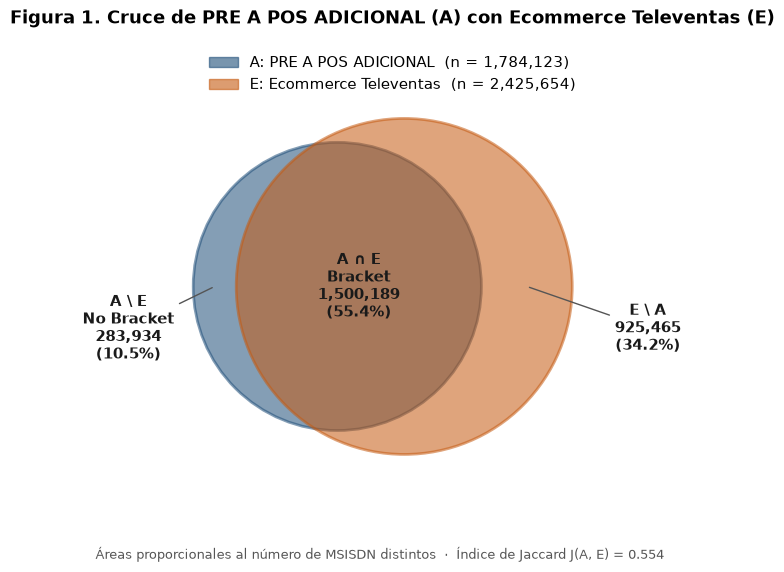
\includegraphics[width=0.78\textwidth]{img/fig1.png}
\caption{Cruce de PRE A POS ADICIONAL ($A$) con Ecommerce Televentas ($E$). Áreas proporcionales al número de MSISDN distintos; $J(A,E)=0.554$.}\label{fig:venn1}
\end{figure}

\section{Exportación de la base No Bracket}
\needspace{8\baselineskip}
\captionof{listing}{Exportación de \cod{base no bracket.csv}}\label{lst:exp-nb}
\inputminted{python}{code/cell18.py}

Se exportaron 283,934 registros a \cod{base no bracket.csv}, con codificación \cod{utf-8-sig} y sin índice.

%% ------------------------------------------------------------------
\chapter{Cruce II: Pre a Home}\label{chap:prehome}
%% ------------------------------------------------------------------

\textbf{Definición:} $\text{Pre a Home}=H\setminus E$ (ecuación~\ref{eq:prehome}).

Se buscan los registros de \emph{PRE A HOME} que \textbf{no} están en \emph{Ecommerce Televentas}. A este conjunto se le llama \textbf{base Pre a Home}.

\needspace{8\baselineskip}
\captionof{listing}{Cruce de $H$ contra $E$ por MSISDN}\label{lst:cruce2}
\inputminted{python}{code/cell20.py}

\begin{table}[H]
\centering
\caption{Resultado del cruce $H$ contra $E$}\label{tab:cruce2}
\small
\begin{tabularx}{0.9\textwidth}{@{}Xr@{}}
\toprule
\tablehead \hd{Medida} & \hd{MSISDN}\\
\midrule
$\card{H\setminus E}$: de \cod{df1} que no están en \cod{df4} (Pre a Home) & \textbf{1,162,392} \\
$\card{E\setminus H}$: de \cod{df4} que no están en \cod{df1} & 2,425,654 \\
Total de MSISDN distintos que no coinciden & 3,588,046 \\
\bottomrule
\end{tabularx}
\end{table}

\textbf{Resultado.} $\card{H\setminus E}=1{,}162{,}392$ registros en la base Pre a Home.

\begin{alerta}
Como $\card{E\setminus H}=\card{E}=2{,}425{,}654$, la intersección es vacía ($H\cap E=\varnothing$) y la base Pre a Home coincide con la totalidad de \cod{df1}: el cruce no excluye ningún registro. Una intersección nula entre dos bases de más de un millón de líneas conviene validarla (por ejemplo, confirmando que el formato del MSISDN es comparable entre ambas fuentes).
\end{alerta}

\subsection*{Diagrama de Venn}
\needspace{8\baselineskip}
\captionof{listing}{Construcción de la figura~\ref{fig:venn2}}\label{lst:venn2}
\inputminted{python}{code/cell22.py}

\begin{figure}[H]
\centering
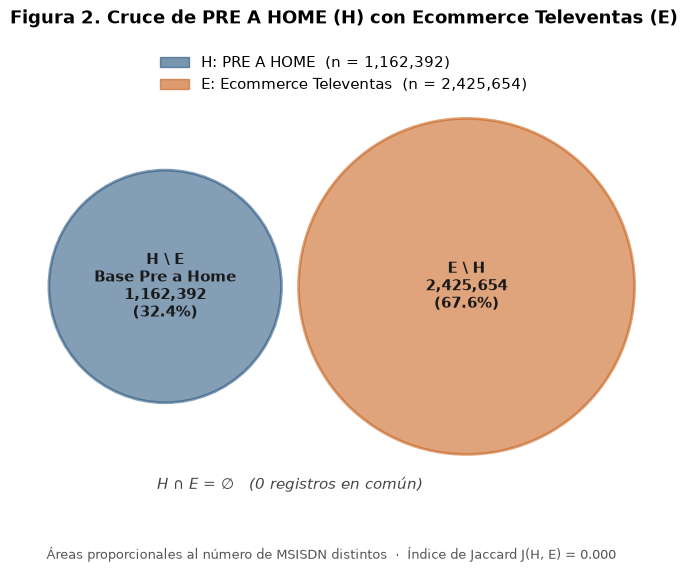
\includegraphics[width=0.7\textwidth]{img/fig2.png}
\caption{Cruce de PRE A HOME ($H$) con Ecommerce Televentas ($E$). Los conjuntos son disjuntos: $H\cap E=\varnothing$.}\label{fig:venn2}
\end{figure}

\section{Exportación de la base Pre a Home}
\needspace{8\baselineskip}
\captionof{listing}{Exportación de \cod{base pre a home.csv}}\label{lst:exp-ph}
\inputminted{python}{code/cell24.py}

Se exportaron 1,162,392 registros a \cod{base pre a home.csv}.

%% ------------------------------------------------------------------
\chapter{Cruce III: Bracket}\label{chap:bracket}
%% ------------------------------------------------------------------

\textbf{Definición:} $\text{Bracket}=A\cap E$ (ecuación~\ref{eq:bracket}).

Se buscan los registros que \textbf{sí} se cruzan entre \emph{PRE A POS ADICIONAL} y \emph{Ecommerce Televentas}. A este conjunto se le llama \textbf{Brackets}.

\needspace{8\baselineskip}
\captionof{listing}{Intersección $A\cap E$ y extracción de los registros completos}\label{lst:cruce3}
\inputminted{python}{code/cell26.py}

\textbf{Resultado.} $\card{A\cap E}=1{,}500{,}189$ registros Bracket, valor que coincide con la región central de la figura~\ref{fig:venn1}.

\section{Unión de las bases cruzadas (\emph{inner join})}
Se unen, por MSISDN, los registros de $A$ y de $E$ que sí cruzan (\cod{df3_cruce} y \cod{df4_cruce}), con los sufijos \cod{_prepos} y \cod{_ecommerce} para las columnas de igual nombre. El resultado (\cod{df_merge}) tiene \textbf{1,500,189 filas $\times$ 74 columnas}; que el número de filas sea igual a $\card{A\cap E}$ confirma una relación uno a uno entre las llaves.

\needspace{8\baselineskip}
\captionof{listing}{\emph{Inner join} entre $A$ y $E$}\label{lst:merge}
\inputminted{python}{code/cell28.py}

%% ------------------------------------------------------------------
\chapter{Consolidación de la base final}\label{chap:consol}
%% ------------------------------------------------------------------

\section{Unión de PRE A POS limpia y de inicio de mes}\label{sec:union-pos}
Se carga la base $P'$ (\cod{df5}) y se concatena con $P$ (\cod{df2}): $\text{df\_nuevo}=P\concat P'$, que resulta en \textbf{2,208,612 filas $\times$ 13 columnas}. \texttt{pandas} emite un \cod{DtypeWarning} por tipos mixtos en la columna \cod{SUM_RVNU_TOT}.

\needspace{6\baselineskip}
\captionof{listing}{Carga de $P'$ (\cod{df5})}\label{lst:df5}
\inputminted{python}{code/cell31.py}

\needspace{6\baselineskip}
\captionof{listing}{Concatenación $P\concat P'$}\label{lst:dfnuevo}
\inputminted{python}{code/cell32.py}

\section{Unión de \cod{df_nuevo} y \cod{df_merge}}
Se concatenan las filas de la base PRE A POS consolidada (\cod{df_nuevo}) con las de los Bracket (\cod{df_merge}), con lo que se obtiene \cod{df_final}: $2{,}208{,}612+1{,}500{,}189=3{,}708{,}801$ filas.

\needspace{6\baselineskip}
\captionof{listing}{Construcción de \texttt{df\_final}}\label{lst:dffinal}
\inputminted{python}{code/cell35.py}

\section{Selección del bracket de menor valor}\index{bracket de menor valor}
Para cada fila de \cod{df_final} se extrae el precio inicial de los planes recomendados (\cod{ID_PLAN_RECOMMENDED_1} e \cod{ID_PLAN_RECOMMENDED_2}) y se conserva el \textbf{menor}. El resultado es \cod{df_msisdn_bracket}, con el MSISDN, el bracket asignado y el total de registros de su categoría, junto con \cod{df_conteo_brackets}, que resume una fila por bracket.

\needspace{10\baselineskip}
\captionof{listing}{Selección del bracket de menor valor y resumen por bracket}\label{lst:seleccion}
\inputminted{python}{code/cell37.py}

\section{Exportación de los brackets}
Se genera un archivo CSV por cada categoría de bracket en la carpeta \cod{resultados bases}, con las columnas \cod{MSISDN}, \cod{bracket} y \cod{cantidad_registros_bracket}. Las filas sin bracket asignado no se exportan.

\needspace{6\baselineskip}
\captionof{listing}{Exportación de un archivo por bracket}\label{lst:exp-br}
\inputminted{python}{code/cell39.py}

\section{Verificación de las cantidades exportadas}
Se vuelven a leer los archivos exportados y se compara su número de filas con el esperado según \cod{df_msisdn_bracket}. La verificación resulta \textbf{exitosa en las nueve categorías}.

\needspace{10\baselineskip}
\captionof{listing}{Verificación de las cantidades exportadas}\label{lst:verif}
\inputminted{python}{code/cell41.py}

\begin{table}[H]
\centering
\caption{Verificación de las cantidades exportadas por bracket}\label{tab:verif}
\small
\begin{tabularx}{0.75\textwidth}{@{}CRRC@{}}
\toprule
\tablehead \hd{Bracket} & \hd{Esperado} & \hd{En archivo} & \hd{Correcto}\\
\midrule
19.9 & 1,539,689 & 1,539,689 & \ok \\
24.9 & 205,058   & 205,058   & \ok \\
29.9 & 106,111   & 106,111   & \ok \\
34.9 & 205,911   & 205,911   & \ok \\
39.9 & 66,843    & 66,843    & \ok \\
43.9 & 107,129   & 107,129   & \ok \\
47.9 & 136,882   & 136,882   & \ok \\
53.9 & 124,798   & 124,798   & \ok \\
69.9 & 112,074   & 112,074   & \ok \\
\bottomrule
\end{tabularx}
\end{table}

\section{Resultados: distribución de los brackets}\label{sec:resultados}
Las bases \cod{df_final} y \cod{df_msisdn_bracket} ya no residen en memoria. Para que el notebook conserve el resultado sin necesidad de recalcularlas, las cifras de las secciones anteriores se registran tal como fueron obtenidas en la ejecución, junto con una validación interna de consistencia.

\begin{table}[H]
\centering
\caption{Indicadores de la base final \cod{df_final}}\label{tab:indicadores}
\small
\begin{tabularx}{0.8\textwidth}{@{}Xr@{}}
\toprule
\tablehead \hd{Indicador} & \hd{Valor}\\
\midrule
Filas de \cod{df_final}                          & 3,708,801 \\
Filas con bracket asignado                       & 2,604,495 (\pct{70.2}) \\
Filas sin bracket (ambos planes vacíos)          & 1,104,306 (\pct{29.8}) \\
Categorías de bracket                            & 9 \\
Rango de brackets                                & 19.9 a 69.9 \\
\bottomrule
\end{tabularx}
\end{table}

\begin{table}[H]
\centering
\caption{Registros por bracket y archivo exportado}\label{tab:brackets}
\footnotesize
\begin{tabularx}{\textwidth}{@{}cRRRRlc@{}}
\toprule
\tablehead \hd{Bracket} & \hd{Registros} & \hd{\% con bracket} & \hd{\% acum.} & \hd{\% de \texttt{df\_final}} & \hd{Archivo exportado} & \hd{Verif.}\\
\midrule
19.9 & 1,539,689 & \pct{59.1}  & \pct{59.1}  & \pct{41.5} & \cod{bracket_19.9.csv} & \ok \\
24.9 & 205,058   & \pct{7.9}   & \pct{67.0}  & \pct{5.5}  & \cod{bracket_24.9.csv} & \ok \\
29.9 & 106,111   & \pct{4.1}   & \pct{71.1}  & \pct{2.9}  & \cod{bracket_29.9.csv} & \ok \\
34.9 & 205,911   & \pct{7.9}   & \pct{79.0}  & \pct{5.6}  & \cod{bracket_34.9.csv} & \ok \\
39.9 & 66,843    & \pct{2.6}   & \pct{81.5}  & \pct{1.8}  & \cod{bracket_39.9.csv} & \ok \\
43.9 & 107,129   & \pct{4.1}   & \pct{85.6}  & \pct{2.9}  & \cod{bracket_43.9.csv} & \ok \\
47.9 & 136,882   & \pct{5.3}   & \pct{90.9}  & \pct{3.7}  & \cod{bracket_47.9.csv} & \ok \\
53.9 & 124,798   & \pct{4.8}   & \pct{95.7}  & \pct{3.4}  & \cod{bracket_53.9.csv} & \ok \\
69.9 & 112,074   & \pct{4.3}   & \pct{100.0} & \pct{3.0}  & \cod{bracket_69.9.csv} & \ok \\
\midrule
\textbf{Total} & \textbf{2,604,495} & \textbf{\pct{100.0}} & & \textbf{\pct{70.2}} & & \\
\bottomrule
\end{tabularx}
\end{table}

\needspace{10\baselineskip}
\captionof{listing}{Tabla de distribución de brackets con control de consistencia}\label{lst:tabla-br}
\inputminted{python}{code/cell43.py}

\needspace{10\baselineskip}
\captionof{listing}{Construcción de la figura~\ref{fig:brackets}}\label{lst:fig-br}
\inputminted{python}{code/cell45.py}

\begin{figure}[H]
\centering
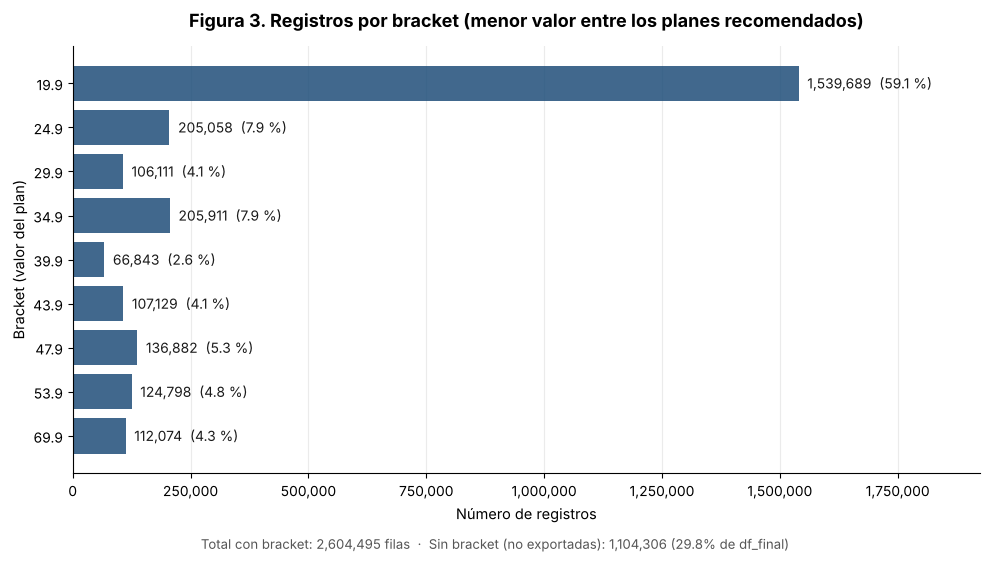
\includegraphics[width=0.95\textwidth]{img/fig3.png}
\caption{Registros por bracket (menor valor entre los planes recomendados). Total con bracket: 2,604,495 filas; sin bracket (no exportadas): 1,104,306 (\pct{29.8} de \texttt{df\_final}).}\label{fig:brackets}
\end{figure}

\subsection*{Lectura de resultados}
\begin{itemize}
  \item El bracket \textbf{19.9} concentra 1,539,689 registros, es decir, el \pct{59.1} de las filas con bracket asignado y más de siete veces el volumen del siguiente bracket (34.9, con 205,911).
  \item Los ocho brackets restantes suman 1,064,806 registros (\pct{40.9}), distribuidos entre 66,843 (bracket 39.9) y 205,911 (bracket 34.9).
  \item Las nueve cantidades exportadas coinciden con las esperadas (tabla~\ref{tab:verif}), por lo que no hay pérdida ni duplicación de filas entre la base en memoria y los archivos.
  \item Las \textbf{1,104,306 filas sin bracket} (\pct{29.8} de \cod{df_final}) no tienen ningún plan recomendado y no forman parte de los archivos de salida (véase el capítulo~\ref{chap:limit}).
\end{itemize}

%% ------------------------------------------------------------------
\chapter{Criterio de selección del bracket}\label{chap:criterio}
%% ------------------------------------------------------------------

Sobre \cod{df_final}, para cada MSISDN se comparan las dos columnas con los brackets recomendados (\cod{ID_PLAN_RECOMMENDED_1} e \cod{ID_PLAN_RECOMMENDED_2}) y se conserva el de \textbf{menor valor}. Si $p_1(m)$ y $p_2(m)$ son los precios extraídos de ambos planes para la fila $m$, el bracket asignado es
\begin{equation}
  \text{bracket}(m)=\min\{\,p_1(m),\,p_2(m)\,\},
\end{equation}
ignorando los valores faltantes. La implementación está en el listado~\ref{lst:seleccion} y opera de la siguiente forma:
\begin{enumerate}
  \item Se extrae de cada identificador de plan su precio inicial (primer valor numérico, con o sin decimales) y se convierte a número.
  \item Se toma el mínimo por fila (\cod{min(axis=1)}), que ignora los valores faltantes; si ambas columnas están vacías, el bracket queda sin asignar (\cod{NaN}).
  \item Se agrega a cada fila el total de registros de su bracket y se exporta un archivo por categoría, cuyas cantidades se validan contra la base en memoria.
\end{enumerate}

\textbf{Resultado.} Se obtienen \textbf{9 categorías de bracket} (19.9, 24.9, 29.9, 34.9, 39.9, 43.9, 47.9, 53.9 y 69.9) con 2,604,495 filas asignadas; el detalle se presenta en la sección~\ref{sec:resultados}.

\begin{alerta}[Nota metodológica]
Actualmente no existen métodos de imputación de datos faltantes, aspecto importante de revisar. Como consecuencia, las 1,104,306 filas de \cod{df_final} que no tienen ninguno de los dos planes recomendados quedan sin bracket y no se exportan.
\end{alerta}

%% ------------------------------------------------------------------
\chapter{Verificación de consistencia y resumen}\label{chap:verif}
%% ------------------------------------------------------------------

\section{Identidades de partición}
\begin{table}[H]
\centering
\caption{Identidades de partición verificadas}\label{tab:identidades}
\small
\begin{tabularx}{\textwidth}{@{}>{\raggedright\arraybackslash}p{4.4cm}Xc@{}}
\toprule
\tablehead \hd{Identidad} & \hd{Cálculo} & \hd{Estado}\\
\midrule
$\card{A}=\card{A\setminus E}+\card{A\cap E}$ & 283,934 + 1,500,189 = 1,784,123 (= registros de \cod{df3}) & \ok \\
$\card{E}=\card{E\setminus A}+\card{A\cap E}$ & 925,465 + 1,500,189 = 2,425,654 (= registros de \cod{df4}) & \ok \\
$\card{H}=\card{H\setminus E}+\card{H\cap E}$ & 1,162,392 + 0 = 1,162,392 (= registros de \cod{df1}) & \ok \\
$\card{A\bowtie E}=\card{A\cap E}$ & 1,500,189 = 1,500,189 & \ok \\
Filas con bracket + sin bracket = filas de \cod{df_final} & 2,604,495 + 1,104,306 = 3,708,801 & \ok \\
Suma de los 9 brackets = filas con bracket & 1,539,689 + 205,058 + 106,111 + 205,911 + 66,843 + 107,129 + 136,882 + 124,798 + 112,074 = 2,604,495 & \ok \\
Filas esperadas = filas en archivo (por bracket) & 9 de 9 categorías & \ok \\
\bottomrule
\end{tabularx}
\end{table}

Como los conteos de MSISDN distintos coinciden con el número de registros de cada fuente, \textbf{MSISDN funciona como llave sin duplicados} en $H$, $A$ y $E$.

\section{Medidas de asociación entre $A$ y $E$}\index{indice de Jaccard@índice de Jaccard}
\begin{itemize}
  \item Proporción de $A$ contenida en $E$: \textbf{\pct{84.1}}.
  \item Proporción de $E$ contenida en $A$: \textbf{\pct{61.8}}.
  \item Índice de Jaccard:
\end{itemize}
\begin{equation}
  J(A,E)=\frac{\card{A\cap E}}{\card{A\cup E}}=\frac{1{,}500{,}189}{2{,}709{,}588}\approx 0.554
\end{equation}

\section{Resumen de resultados}
\begin{table}[H]
\centering
\caption{Resumen de bases generadas y salidas}\label{tab:resumen}
\footnotesize
\begin{tabularx}{\textwidth}{@{}lcrX@{}}
\toprule
\tablehead \hd{Base} & \hd{Definición} & \hd{Registros} & \hd{Salida}\\
\midrule
No Bracket                & $A\setminus E$ & 283,934   & \cod{base no bracket.csv} \\
Pre a Home                & $H\setminus E$ & 1,162,392 & \cod{base pre a home.csv} \\
Bracket                   & $A\cap E$      & 1,500,189 & \cod{df_merge} (insumo de \cod{df_final}) \\
PRE A POS consolidada     & $P\concat P'$  & 2,208,612 & \cod{df_nuevo} (insumo de \cod{df_final}) \\
Base final                & \cod{df_nuevo} $\concat$ \cod{df_merge} & 3,708,801 & \cod{df_final} (insumo de la selección de bracket) \\
Filas con bracket asignado & mín. de los planes recomendados & 2,604,495 & 9 archivos \cod{bracket_<valor>.csv} \\
Filas sin bracket         & ambos planes vacíos & 1,104,306 & No se exportan \\
\bottomrule
\end{tabularx}
\end{table}

\section{Conclusiones}
\begin{enumerate}
  \item El proceso es \textbf{trazable y consistente}: todas las identidades de partición se cumplen y los archivos exportados reproducen exactamente los conteos esperados.
  \item La segmentación entrega tres productos: \textbf{No Bracket} (283,934), \textbf{Pre a Home} (1,162,392) y \textbf{Bracket}, este último consolidado con PRE A POS y distribuido en nueve categorías de valor.
  \item La distribución está \textbf{muy concentrada} en el bracket de menor valor (19.9), con el \pct{59.1} de las filas con bracket.
  \item Los principales riesgos (filas sin bracket, intersección vacía entre $H$ y $E$, unicidad del MSISDN y ausencia de persistencia intermedia) se describen en el capítulo siguiente, junto con las acciones recomendadas.
\end{enumerate}

%% ------------------------------------------------------------------
\chapter{Limitaciones y recomendaciones}\label{chap:limit}
%% ------------------------------------------------------------------

\begin{table}[H]
\centering
\caption{Limitaciones identificadas y acciones recomendadas}\label{tab:limit}
\footnotesize
\renewcommand{\arraystretch}{1.3}
\begin{tabularx}{\textwidth}{@{}>{\sffamily\bfseries\color{navy}\raggedright\arraybackslash}p{2.9cm}XX@{}}
\toprule
\tablehead \hd{Aspecto} & \hd{Hallazgo} & \hd{Recomendación}\\
\midrule
Datos faltantes sin imputar & Al concatenar, las filas provenientes de PRE A POS (\cod{df2}) quedan con valores faltantes en columnas como \cod{PERIODO}, \cod{ANTIGUEDAD} y \cod{REGIONAL}. & Definir un criterio de imputación o de exclusión. \\
Tipos mixtos & \texttt{pandas} advirtió tipos mixtos en \cod{PERFIL} (\cod{df4}) y \cod{SUM_RVNU_TOT} (\cod{df5}). & Fijar \cod{dtype} explícitos o usar \cod{low_memory=False} al leer. \\
Validación de $H\cap E=\varnothing$ & La intersección entre PRE A HOME y Ecommerce Televentas resultó vacía. & Confirmar que el formato del MSISDN es equivalente en ambas bases antes de dar por válido el resultado. \\
Normalización repetida & La limpieza del MSISDN se reescribe en varias celdas. & Centralizarla en una función para reducir el riesgo de inconsistencias. \\
Rutas locales & Las rutas de lectura son absolutas (Windows) y la carpeta \cod{resultados bases} es relativa al directorio de trabajo. & Parametrizar las rutas para reproducir el proceso en otro equipo. \\
Filas sin bracket & 1,104,306 filas de \cod{df_final} (\pct{29.8}) no tienen ninguno de los dos planes recomendados y quedan fuera de la exportación. La cifra coincide exactamente con el número de registros de una de las dos fuentes PRE A POS (1,104,306). & Revisar qué porción de \cod{df_nuevo} incorpora los planes recomendados. \\
Unicidad del MSISDN en \cod{df_final} & La concatenación de $P$, $P'$ y el \emph{inner join} no garantiza un MSISDN por fila (por ejemplo, una misma línea presente en ambas versiones de PRE A POS). Los 2,604,495 registros con bracket son filas y no necesariamente líneas distintas. & Validar \cod{df_msisdn_bracket["MSISDN"].is_unique} antes de entregar los archivos. \\
Extracción del precio del plan & El bracket se obtiene tomando el primer valor numérico del identificador del plan. & Contrastarlo contra el catálogo oficial de planes para descartar identificadores con numeración distinta al precio. \\
Persistencia de la base consolidada & \cod{df_final} y \cod{df_msisdn_bracket} no se guardan en disco, por lo que cualquier ajuste exige recalcular todo el proceso. & Persistir \cod{df_msisdn_bracket} (por ejemplo, en formato Parquet) como insumo intermedio. \\
\bottomrule
\end{tabularx}
\end{table}

%% ==================================================================
%%  ANEXOS
%% ==================================================================
\appendix

%% ------------------------------------------------------------------
\chapter{Script consolidado}\label{anx:script}
%% ------------------------------------------------------------------
Se reúnen a continuación, en orden de ejecución, las celdas de código del notebook. Se omiten las dos celdas que solo muestran un \emph{DataFrame} (\cod{df_merge} y \cod{df_nuevo}). Las funciones auxiliares de la figura de Venn (\cod{diagrama_venn}) figuran completas en este anexo.

\begin{nota}[Reproducibilidad]
Las rutas de lectura son absolutas y propias del equipo donde se ejecutó el proceso (Windows). Para reproducirlo en otro equipo deben ajustarse a la ubicación local de los archivos de origen (véase el capítulo~\ref{chap:limit}).
\end{nota}

\captionof{listing}{Script consolidado del proceso}\label{lst:script}
\inputminted[linenos,numbersep=7pt]{python}{code/script_completo.py}

%% ------------------------------------------------------------------
\chapter{Salidas de ejecución registradas}\label{anx:salidas}
%% ------------------------------------------------------------------
Se transcriben las salidas de texto producidas por el notebook, sin modificación. No se reproducen las vistas previas de los \emph{DataFrame} para no exponer registros individuales.

\section{Volumetría de las fuentes}
\begin{minted}{text}
1162392
1104306
1784123

C:\Users\danie\AppData\Local\Temp\ipykernel_7960\2106715918.py:1: DtypeWarning: Columns (25: PERFIL) have mixed types. Specify dtype option on import or set low_memory=False.
  df4=pd.read_csv(r"C:\Users\danie\Downloads\Migra Tigo\Ecomerce televentas.csv")
2425654
\end{minted}

\section{Cruce I: No Bracket}
\begin{minted}{text}
MSISDN de df4 que no están en df3: 925,465
MSISDN de df3 que no están en df4: 283,934
Total de MSISDN distintos que no coinciden: 1,209,399

Registros exportados: 283,934
Archivo guardado en: C:\Users\danie\Downloads\resultados bases\base no bracket.csv
\end{minted}

\section{Cruce II: Pre a Home}
\begin{minted}{text}
MSISDN de df1 que no están en df4: 1,162,392
MSISDN de df4 que no están en df1: 2,425,654
Total de MSISDN distintos que no coinciden: 3,588,046

Registros exportados: 1,162,392
Archivo guardado en: C:\Users\danie\Downloads\resultados bases\base pre a home.csv
\end{minted}

\section{Cruce III: Bracket e \emph{inner join}}
\begin{minted}{text}
Cantidad que sí cruzan entre df3 y df4: 1,500,189
Registros unidos: 1,500,189
\end{minted}

\section{Consolidación}
\begin{minted}{text}
C:\Users\danie\AppData\Local\Temp\ipykernel_7960\4078152688.py:1: DtypeWarning: Columns (4: SUM_RVNU_TOT) have mixed types. Specify dtype option on import or set low_memory=False.
  df5=pd.read_csv(r"C:\Users\danie\Downloads\Migra Tigo\PRE A POS.csv")
\end{minted}

Dimensiones registradas: \cod{df_merge}, 1,500,189 filas $\times$ 74 columnas; \cod{df_nuevo}, 2,208,612 filas $\times$ 13 columnas; \cod{df_final}, 3,708,801 filas.

\section{Resumen por bracket}
\begin{minted}{text}
   bracket  cantidad_registros
0     19.9             1539689
1     24.9              205058
2     29.9              106111
3     34.9              205911
4     39.9               66843
5     43.9              107129
6     47.9              136882
7     53.9              124798
8     69.9              112074
\end{minted}

\section{Exportación y verificación de los brackets}
\begin{minted}{text}
Guardado: resultados bases\bracket_19.9.csv
Guardado: resultados bases\bracket_24.9.csv
Guardado: resultados bases\bracket_29.9.csv
Guardado: resultados bases\bracket_34.9.csv
Guardado: resultados bases\bracket_39.9.csv
Guardado: resultados bases\bracket_43.9.csv
Guardado: resultados bases\bracket_47.9.csv
Guardado: resultados bases\bracket_53.9.csv
Guardado: resultados bases\bracket_69.9.csv

         esperado  en_archivo  correcto
bracket                                
19.9      1539689     1539689      True
24.9       205058      205058      True
29.9       106111      106111      True
34.9       205911      205911      True
39.9        66843       66843      True
43.9       107129      107129      True
47.9       136882      136882      True
53.9       124798      124798      True
69.9       112074      112074      True

¿Todas las cantidades coinciden? True
\end{minted}

\section{Control de consistencia final}
\begin{minted}{text}
Total con bracket asignado :  2,604,495  (70.2% de df_final)
Total sin bracket          :  1,104,306  (29.8% de df_final)
Total de filas df_final    :  3,708,801
\end{minted}

%% ------------------------------------------------------------------
\chapter{Catálogo de archivos de salida}\label{anx:catalogo}
%% ------------------------------------------------------------------
Todos los archivos se escriben en la carpeta \cod{resultados bases} con \cod{index=False} y codificación \cod{utf-8-sig}.

\begin{table}[H]
\centering
\caption{Archivos generados por el proceso}\label{tab:catalogo}
\footnotesize
\begin{tabularx}{\textwidth}{@{}>{\ttfamily}p{4.1cm}rXl@{}}
\toprule
\tablehead \hd{Archivo} & \hd{Filas} & \hd{Contenido} & \hd{Origen}\\
\midrule
base no bracket.csv & 283,934 & Registros completos de PRE A POS ADICIONAL ausentes en Ecommerce Televentas & \cod{df3}, $A\setminus E$ \\
base pre a home.csv & 1,162,392 & Registros completos de PRE A HOME ausentes en Ecommerce Televentas & \cod{df1}, $H\setminus E$ \\
bracket\_19.9.csv & 1,539,689 & \cod{MSISDN}, \cod{bracket}, \cod{cantidad_registros_bracket} & \cod{df_msisdn_bracket} \\
bracket\_24.9.csv & 205,058 & ídem & \cod{df_msisdn_bracket} \\
bracket\_29.9.csv & 106,111 & ídem & \cod{df_msisdn_bracket} \\
bracket\_34.9.csv & 205,911 & ídem & \cod{df_msisdn_bracket} \\
bracket\_39.9.csv & 66,843 & ídem & \cod{df_msisdn_bracket} \\
bracket\_43.9.csv & 107,129 & ídem & \cod{df_msisdn_bracket} \\
bracket\_47.9.csv & 136,882 & ídem & \cod{df_msisdn_bracket} \\
bracket\_53.9.csv & 124,798 & ídem & \cod{df_msisdn_bracket} \\
bracket\_69.9.csv & 112,074 & ídem & \cod{df_msisdn_bracket} \\
\bottomrule
\end{tabularx}
\end{table}

%% ------------------------------------------------------------------
\chapter{Glosario}\label{anx:glosario}
%% ------------------------------------------------------------------
\begin{description}[style=nextline,leftmargin=1.2cm]
  \item[MSISDN]\index{MSISDN} Número de línea móvil; llave de identificación de cada registro.
  \item[Bracket]\index{Bracket} Categoría de valor del plan recomendado; se asigna como el menor precio entre los dos planes recomendados de la línea.
  \item[No Bracket]\index{No Bracket} Registros de PRE A POS ADICIONAL ausentes en Ecommerce Televentas ($A\setminus E$).
  \item[Pre a Home]\index{Pre a Home} Registros de PRE A HOME ausentes en Ecommerce Televentas ($H\setminus E$).
  \item[Inner join]\index{inner join} Unión que conserva únicamente las filas cuya llave está presente en ambas tablas.
  \item[Índice de Jaccard]\index{indice de Jaccard@índice de Jaccard} Cociente entre el tamaño de la intersección y el de la unión de dos conjuntos.
  \item[Diagrama de Venn]\index{diagrama de Venn} Representación gráfica de dos conjuntos; en este documento, con áreas proporcionales a su cardinalidad.
  \item[Imputación]\index{imputacion@imputación} Reemplazo de valores faltantes por valores estimados según un criterio definido.
  \item[\cod{DtypeWarning}] Advertencia de \texttt{pandas} que indica tipos mixtos en una columna al leer un archivo.
\end{description}

%% ------------------------------------------------------------------
\chapter{Trazabilidad notebook--documento}\label{anx:traza}
%% ------------------------------------------------------------------
\begin{table}[H]
\centering
\caption{Correspondencia entre las secciones del notebook y este documento}\label{tab:traza}
\small
\begin{tabularx}{\textwidth}{@{}lXl@{}}
\toprule
\tablehead \hd{Sección del notebook} & \hd{Contenido} & \hd{Capítulo}\\
\midrule
1 & Carga de las bases de datos & \ref{chap:carga} \\
2 & Volumetría de las fuentes & \ref{chap:carga} \\
3 & Preparación de la llave y utilidades & \ref{chap:llave} \\
4 & Cruce I de No Bracket & \ref{chap:nobracket} \\
5 & Cruce II de Pre a Home & \ref{chap:prehome} \\
6 & Cruce III de Bracket & \ref{chap:bracket} \\
7 & Consolidación de la base final & \ref{chap:consol} \\
8 & Criterio de selección del bracket & \ref{chap:criterio} \\
9 & Verificación de consistencia y resumen & \ref{chap:verif} \\
10 & Limitaciones y recomendaciones & \ref{chap:limit} \\
\bottomrule
\end{tabularx}
\end{table}

%% ==================================================================
%%  BIBLIOGRAFÍA E ÍNDICE
%% ==================================================================
\backmatter
\chapter*{Referencias}
\addcontentsline{toc}{chapter}{Referencias}
\markboth{Referencias}{}
\begin{thebibliography}{9}
\bibitem{mckinney2010} McKinney, W. (2010). Data structures for statistical computing in Python. \emph{Proceedings of the 9th Python in Science Conference}, 56--61.
\bibitem{harris2020} Harris, C. R., et al. (2020). Array programming with NumPy. \emph{Nature}, 585, 357--362.
\bibitem{hunter2007} Hunter, J. D. (2007). Matplotlib: A 2D graphics environment. \emph{Computing in Science \& Engineering}, 9(3), 90--95.
\bibitem{jaccard1912} Jaccard, P. (1912). The distribution of the flora in the alpine zone. \emph{New Phytologist}, 11(2), 37--50.
\bibitem{codd1970} Codd, E. F. (1970). A relational model of data for large shared data banks. \emph{Communications of the ACM}, 13(6), 377--387.
\end{thebibliography}

\clearpage
\printindex

\end{document}
